\chapter{Sprint 4 : Candidatures et Espace Candidat}

\section*{Introduction}

Ce chapitre présente la réalisation du \textbf{sprint 4} de TalentFlow, en lien avec
les user stories US07 et US08 du backlog produit (chapitre~2), du point de vue
\textbf{candidat authentifié}. S'appuyant sur les offres publiées au sprint~3
(chapitre~5), ce sprint couvre l'exploration des postes, le dépôt de candidature
avec upload de CV sur \textbf{Cloudinary}, la gestion du profil, les offres
sauvegardées et le suivi visuel du pipeline de candidatures. Nous présentons
l'objectif, le backlog, l'analyse des cas d'utilisation et les interfaces réalisées.

% ============================================================
\section{Objectif du Sprint}
% ============================================================

L'objectif principal de ce sprint est de fournir un \textbf{portail candidat}
(\texttt{/dashboard}, \texttt{/offres}, \texttt{/applications}, etc.) permettant :

\begin{itemize}
    \item \textbf{Explorer les offres} publiées du tenant : recherche par mots-clés
    et localisation, filtres par type de contrat et catégorie
    (\texttt{OffresView.vue}).

    \item \textbf{Consulter le détail} d'une offre et \textbf{postuler} via un
    formulaire dynamique (\texttt{OffreDetailsApplyView.vue}), incluant les champs
    personnalisés définis au sprint~3 (\texttt{ChampPersonnalise}).

    \item \textbf{Déposer le CV} : le fichier est transmis à l'API .NET qui
    l'héberge sur Cloudinary ; l'URL sécurisée est enregistrée dans
    \texttt{Candidature.CvUrl}.

    \item \textbf{Gérer le profil candidat} (\texttt{CandidateProfile}) : informations
    personnelles, statut de carrière, force du profil.

    \item \textbf{Sauvegarder des offres} en favoris (\texttt{SavedJob}) et les
    retrouver dans l'espace \textit{Saved jobs}.

    \item \textbf{Suivre les candidatures} : statistiques, liste filtrable et
    pipeline Kanban par étape (\texttt{Applied}, \textit{In Review}, \textit{Shortlisted},
    \textit{Interview}, \textit{Accepted}, \textit{Declined}).
\end{itemize}

% ============================================================
\section{Analyse du Sprint 4}
% ============================================================

\subsection{Sprint Backlog}

Le tableau~\ref{tab:backlog_s4} présente les user stories traitées dans ce chapitre
(vue candidat du sprint~4).

\begin{table}[h]
\centering
\renewcommand{\arraystretch}{1.4}
\begin{tabular}{|c|p{8.5cm}|c|}
\hline
\textbf{ID} & \textbf{User Story} & \textbf{Priorité} \\
\hline
US07 & En tant que candidat authentifié, je veux postuler à une offre avec mon CV
(hébergé sur Cloudinary) et compléter le formulaire de candidature. & Haute \\
\hline
US07a & En tant que candidat, je veux explorer les offres publiées, consulter
leur fiche et sauvegarder celles qui m'intéressent (\texttt{SavedJob}). & Haute \\
\hline
US07b & En tant que candidat, je veux gérer mon profil (\texttt{CandidateProfile})
afin d'améliorer ma visibilité auprès des recruteurs. & Haute \\
\hline
US08 & En tant que candidat, je veux suivre l'évolution de mes candidatures
(\texttt{Candidature.Statut}) via un tableau de bord et un pipeline visuel. & Haute \\
\hline
\end{tabular}
\caption{Sprint Backlog du Sprint 4 (espace candidat)}
\label{tab:backlog_s4}
\end{table}

\subsection{Diagramme de Cas d'Utilisation — Sprint 4}

\begin{figure}[ht]
    \centering
    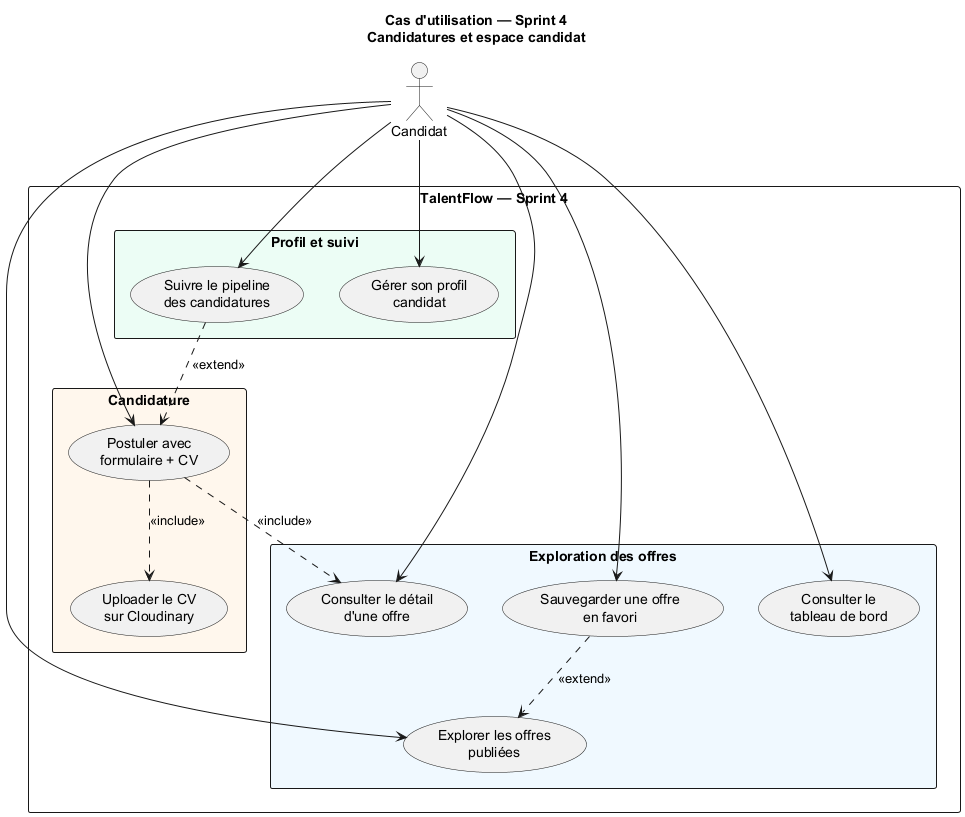
\includegraphics[width=0.95\textwidth]{images/usecase_sprint4.png}
    \caption{Diagramme de cas d'utilisation du Sprint 4}
    \label{fig:uc_sprint4}
\end{figure}

\subsubsection{Description Textuelle des Cas d'Utilisation}

\textbf{Cas d'utilisation : Postuler à une offre avec CV}

\begin{itemize}
    \item \textbf{Acteur principal :} Candidat authentifié
    \item \textbf{Précondition :} offre publiée (\texttt{EstPublie = true}), date limite
    non dépassée, candidat non déjà inscrit sur l'offre.
    \item \textbf{Scénario nominal :}
    \begin{enumerate}
        \item Le candidat ouvre la fiche offre (\texttt{/offres/:id}).
        \item Il renseigne nom, email, portfolio, motivation et dépose un CV
        (PDF, DOCX, DOC ou image, max.\ 10\,Mo).
        \item L'API enregistre la \texttt{Candidature} et uploade le fichier sur
        Cloudinary (\texttt{CvUrl}).
        \item Un message de succès s'affiche ; redirection vers \textit{My Applications}.
    \end{enumerate}
    \item \textbf{Exception :} candidature déjà existante (HTTP 409), date limite
    dépassée (\textit{Candidatures closes}).
\end{itemize}

\textbf{Cas d'utilisation : Suivre le pipeline des candidatures}

\begin{itemize}
    \item \textbf{Acteur principal :} Candidat
    \item \textbf{Scénario nominal :} le candidat consulte \textit{My Applications},
    filtre par statut (\textit{Pending}, \textit{Interview}, \textit{Accepted},
    \textit{Rejected}) et visualise chaque dossier dans la colonne Kanban correspondante.
    \item \textbf{Postcondition :} le statut affiché reflète \texttt{Candidature.Statut}
    mis à jour par le recruteur (traitement côté tenant au sprint~5 et suivants).
\end{itemize}

% ============================================================
\section{Réalisation}
% ============================================================

\subsection{Tableau de Bord Candidat}

Le \textit{Candidate Portal} démarre sur le tableau de bord
(\texttt{CandidatDashboard.vue}, route \texttt{/dashboard}). Des cartes récapitulent
les offres actives et les entretiens à venir ; une section présente les dernières
offres publiées avec accès rapide à la candidature (\textit{Quick Apply}) ; un panneau
de notifications récentes complète la vue d'ensemble.

\begin{figure}[ht]
    \centering
    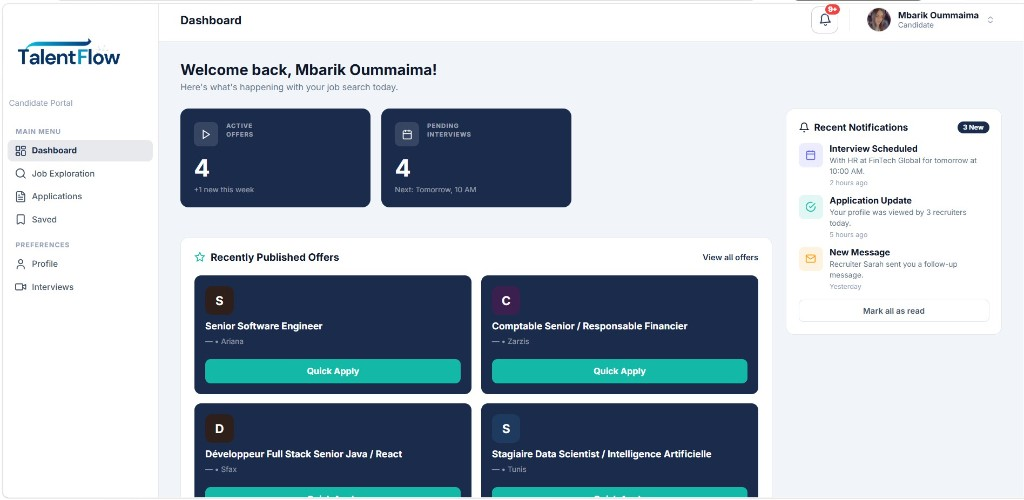
\includegraphics[width=\textwidth]{images/candidate_dashboard.jpg}
    \caption{Tableau de bord du portail candidat}
    \label{fig:candidate_dashboard}
\end{figure}

\subsection{Exploration des Offres}

La page \textit{Job Exploration} (\texttt{OffresView.vue}, \texttt{/offres}) propose
une recherche par titre, compétences ou mots-clés et par localisation. Des filtres
par catégorie (\textit{Full-time}, \textit{Remote}, \textit{IT \& Tech}, etc.) et des
cartes d'offres (entreprise, lieu, type de contrat, date de publication) permettent
d'accéder au détail ou de lancer la candidature. Un panneau latéral affiche la
\textit{Profile Strength} et les compétences tendances.

\begin{figure}[ht]
    \centering
    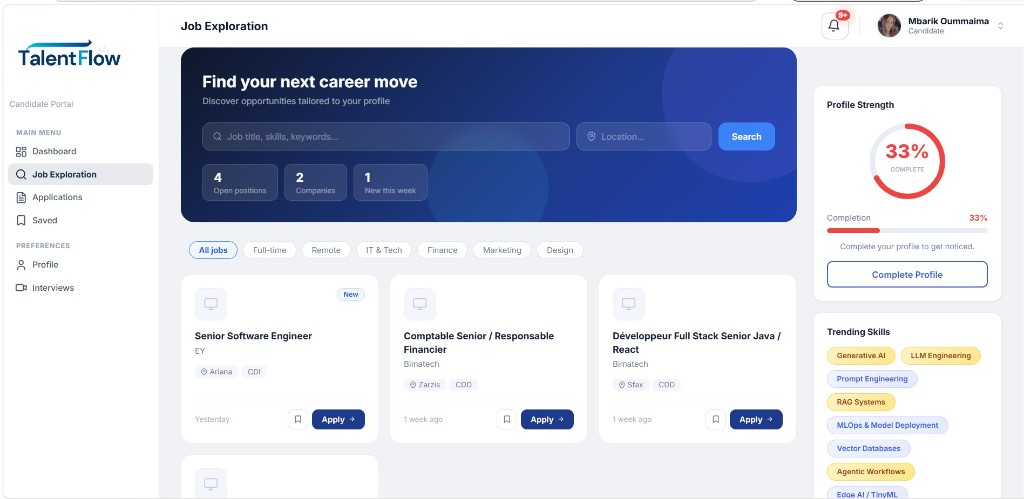
\includegraphics[width=\textwidth]{images/candidate_job_exploration.jpg}
    \caption{Exploration et recherche des offres publiées}
    \label{fig:candidate_job_exploration}
\end{figure}

\subsection{Consultation du Détail d'une Offre}

La route \texttt{/offres/:id} (\texttt{OffreDetailsApplyView.vue}) affiche la fiche
complète : titre, entreprise, localisation, description enrichie, missions et profil
recherché. Le candidat peut revenir à la recherche ou poursuivre vers le formulaire
de candidature dans la même vue.

\begin{figure}[ht]
    \centering
    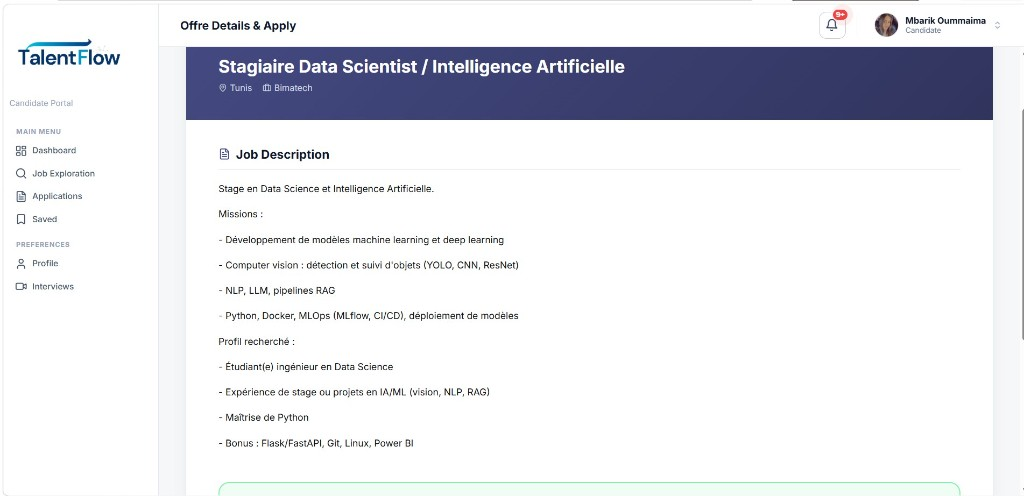
\includegraphics[width=\textwidth]{images/candidate_offer_detail.jpg}
    \caption{Consultation du détail d'une offre avant candidature}
    \label{fig:candidate_offer_detail}
\end{figure}

\subsection{Dépôt de Candidature et Upload CV (Cloudinary)}

Le formulaire de candidature regroupe les champs obligatoires (nom, email), le lien
portfolio, la zone de dépôt CV (glisser-déposer ou sélection de fichier) et la
motivation. À la soumission (\textit{Submit Application}), le frontend envoie un
\texttt{FormData} multipart à l'endpoint de candidature ; le service
\texttt{CandidatService} côté API .NET utilise \texttt{CloudinaryDotNet} pour stocker
le document et persister l'URL dans \texttt{CvUrl}. Les réponses aux champs
personnalisés configurés par le recruteur sont transmises en JSON
(\texttt{champsPersonnalises}).

\begin{figure}[ht]
    \centering
    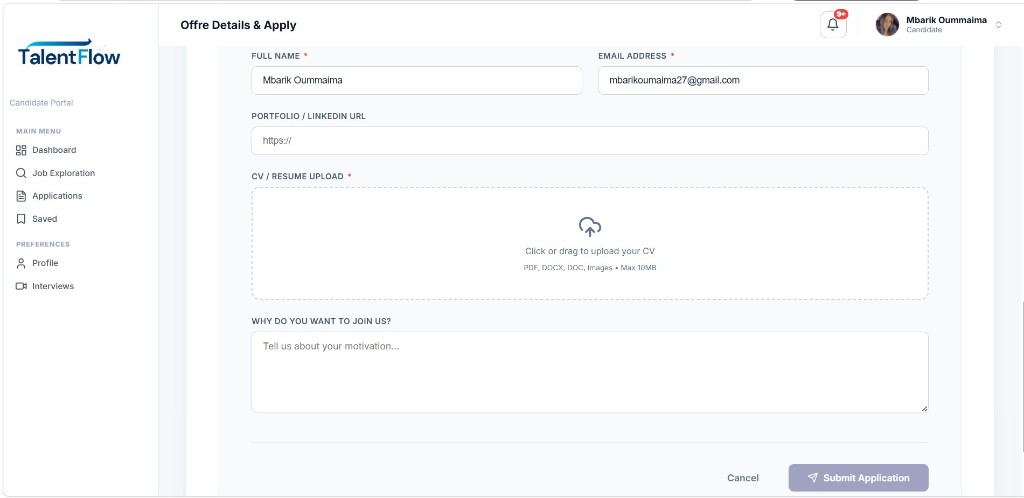
\includegraphics[width=\textwidth]{images/candidate_apply_form.jpg}
    \caption{Formulaire de candidature avec upload de CV}
    \label{fig:candidate_apply_form}
\end{figure}

\subsection{Offres Sauvegardées}

L'écran \textit{Saved jobs} (\texttt{/saved}) liste les offres mises en favori
(\texttt{SavedJob}). Chaque carte rappelle le poste, l'entreprise, la localisation,
le type de contrat et la date de sauvegarde ; l'utilisateur peut retirer une offre
de sa liste.

\begin{figure}[ht]
    \centering
    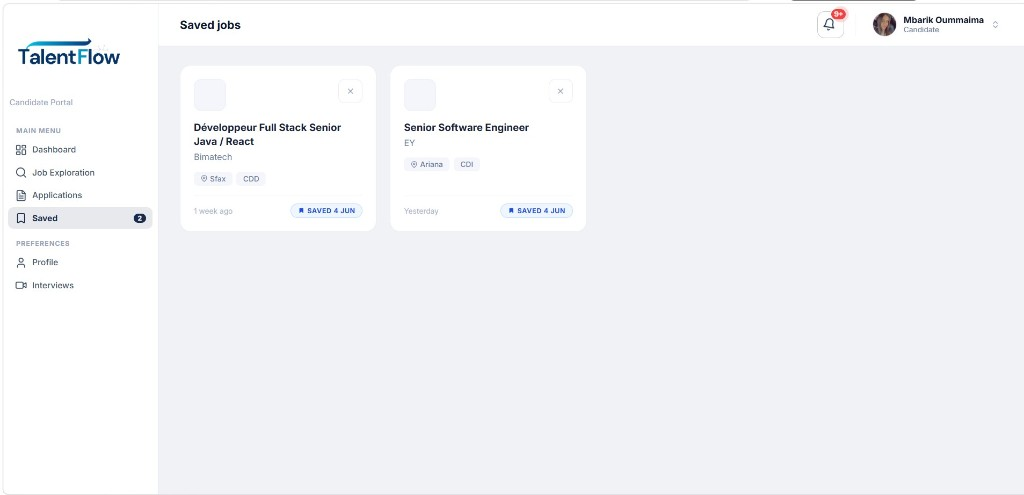
\includegraphics[width=\textwidth]{images/candidate_saved_jobs.jpg}
    \caption{Gestion des offres sauvegardées}
    \label{fig:candidate_saved_jobs}
\end{figure}

\subsection{Profil Candidat}

La page \textit{My Profile} permet de compléter les informations personnelles
(téléphone, localisation, bio), le statut de carrière (\textit{Student},
\textit{Looking for Internship}, etc.), le niveau d'études et la disponibilité.
Un indicateur de \textit{Profile Strength} incite à enrichir le profil pour améliorer
la visibilité.

\begin{figure}[ht]
    \centering
    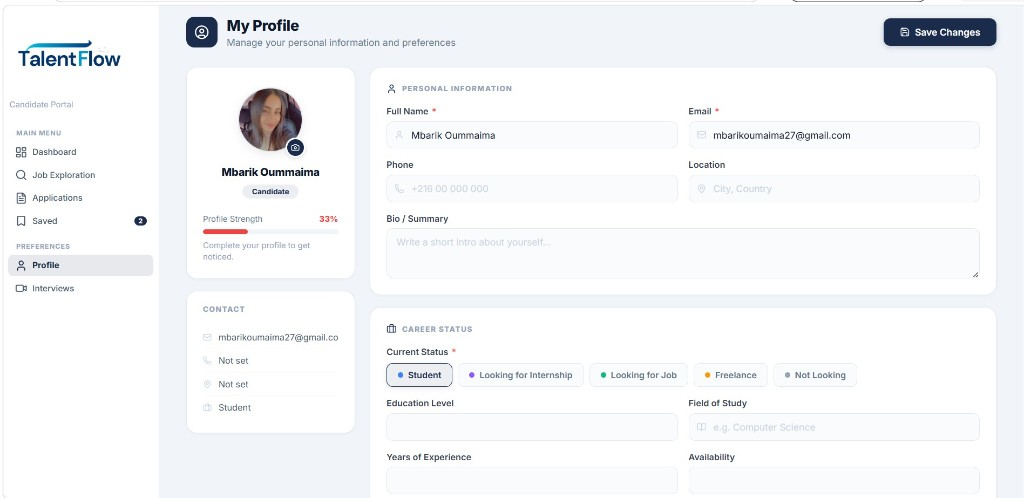
\includegraphics[width=\textwidth]{images/candidate_profile.jpg}
    \caption{Gestion du profil candidat (\texttt{CandidateProfile})}
    \label{fig:candidate_profile}
\end{figure}

\subsection{Pipeline de Suivi des Candidatures}

\textit{My Applications} (\texttt{CandidatApplications.vue}, \texttt{/applications})
combine quatre indicateurs (\textit{Total}, \textit{Pending}, \textit{Accepted},
\textit{Rejected}), une liste filtrable et un \textbf{Application Pipeline} en
colonnes : \textit{Applied}, \textit{In Review}, \textit{Shortlisted},
\textit{Interview}, \textit{Accepted}, \textit{Declined}. Chaque carte affiche le
poste, l'entreprise et, le cas échéant, le score ou la notation attribuée par le
recruteur.

\begin{figure}[ht]
    \centering
    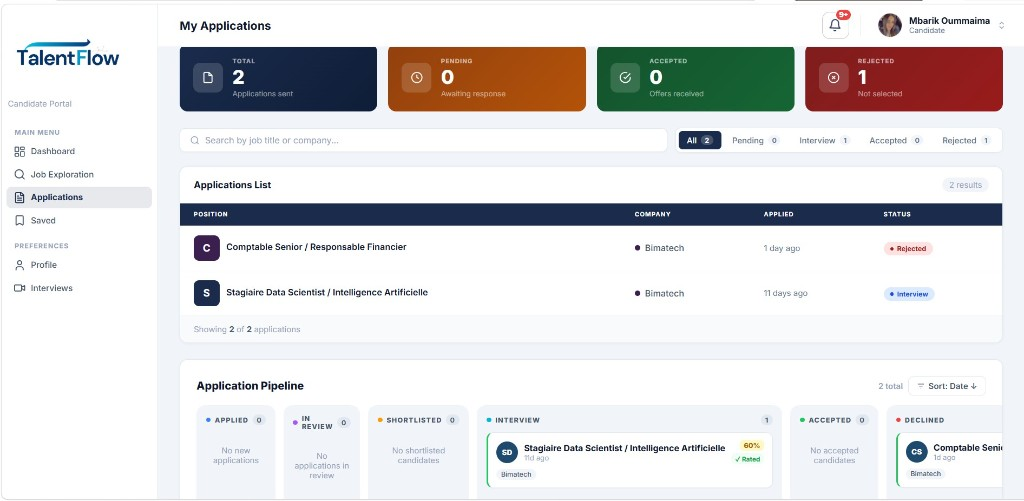
\includegraphics[width=\textwidth]{images/candidate_applications_pipeline.jpg}
    \caption{Suivi des candidatures : liste et pipeline Kanban}
    \label{fig:candidate_applications_pipeline}
\end{figure}

\section*{Conclusion}

Le sprint 4 a livré l'\textbf{espace candidat} de TalentFlow : exploration des
offres, dépôt de candidature avec CV hébergé sur Cloudinary, profil enrichissable,
favoris et suivi visuel du pipeline. Les candidatures sont désormais enregistrées
dans le modèle \texttt{Candidature} et prêtes pour les traitements IA du sprint~5
(extraction CV, scoring et classement sémantique).
